% !TEX root = main.tex
% Main text: abstract through conclusion. Formal assumptions, full statements and proofs are in the appendix.
\begin{abstract}
We prove a learning-time separation between outcome and process supervision in a concrete Transformer. For counting modulo $K$ in a
two-block causal softmax-attention/ReLU Transformer that holds exact executors for both formats, gradient flow from the same small
initialization, on the same trainable parameters, stays near chance for time $\Omega(\mixrate^{-n})$ when trained on the final count, and
reaches positive margins on every recurring transition in time $O(n^{5/2}\log n)$ when trained on the running counts, with the attention routing
fixed. The mechanism is credit contraction: each letter a feature does not read multiplies its correlation with the final count by
$\mixrate<1$, and near initialization the network is built from features that read few letters, whereas a displayed count leaves an
order-one local signal. Experiments drop the theorems' assumptions one at a time, from learned routing to all parameters under AdamW,
other state-tracking tasks and LoRA-tuned Qwen2.5-0.5B; the separation persists at every rung except one object-tracking size.
\end{abstract}

% ===================================================================
\section{Introduction}
\label{sec:intro}

Intermediate supervision often makes reasoning tasks learnable \citep{nye2021scratchpads,wei2022cot,lightman2023verify}, even when the
same network can represent the answer-only solution. We isolate this effect in one task, one architecture and one initialization, and
prove that it is an optimization effect. For counting a query letter modulo $K$ over $n$ letters, a two-block Transformer holds exact
parameters for both the final-answer and the running-count format (\cref{prop:represent}). From the same seed and on the same trainable
parameters, outcome gradient flow stays near chance for time $\Omega(\mixrate^{-n})$ (\cref{thm:outcome-end}), while step gradient flow
reaches positive margins on every recurring transition $s_{t-1},w_t\mapsto s_t$, $t\ge2$, in polynomial time (\cref{thm:joint}); together they give a matched exponential separation
(\cref{cor:matched}).

The mechanism is where the gradient credit lies. Averaging over every letter that a feature does not read contracts its correlation with
the final count by a factor $\mixrate<1$ per letter. Near initialization the network's output is dominated by terms that each read one
letter, and combining more letters costs powers of the initialization scale (\cref{fig:overview}b). A displayed count and the current
letter, by contrast, expose the next update directly:
{\small
\[
\begin{aligned}
 &\text{outcome:}&&\text{hidden letters}\to\text{few-letter features decorrelate}\to\text{tiny credit}\to\text{plateau},\\
 &\text{step:}&&\text{displayed count}\to\text{local innovation}\to\text{accessible credit}\to\text{learned transition}\to\text{solution}.
\end{aligned}
\]
}

\begin{figure}[t]
\centering
%% Figure 1 (pgfplots). Data: results/paper/zero_readout_n16_8k (seeds 42-51, median and 25th-75th percentile band),
%% results/paper/fig2/n8_s42.json (target A_r) and results/paper/exact_spectra/sigma_sweep/s42_sg0.02.txt (Jacobian J_r).
\definecolor{stepc}{HTML}{0072B2}\definecolor{outc}{HTML}{D55E00}\definecolor{theoc}{HTML}{009E73}
\definecolor{modelc}{HTML}{7B4F9E}\definecolor{mutedc}{HTML}{6E6E6E}
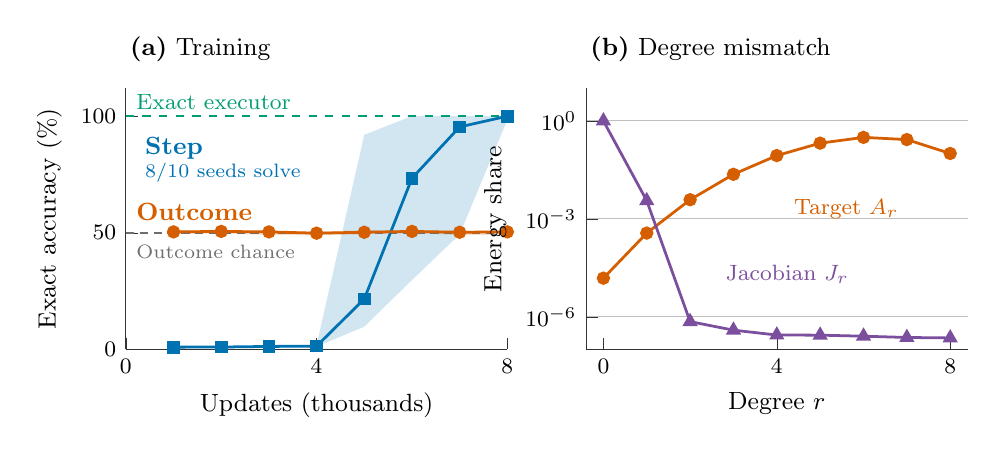
\begin{tikzpicture}
\pgfplotsset{every axis/.style={width=0.53\linewidth, height=4.9cm, axis line style={black!80}, tick style={black!80},
  tick label style={font=\footnotesize}, label style={font=\small}, title style={font=\small, at={(0,1)}, anchor=south west, xshift=-2pt}},
  every axis plot/.append style={line width=1pt}}
\begin{axis}[name=train, title={\textbf{(a)} Training}, xlabel={Updates (thousands)}, ylabel={Exact accuracy (\%)},
  xmin=0, xmax=8, ymin=0, ymax=112, xtick={0,4,8}, ytick={0,50,100}, axis x line*=bottom, axis y line*=left, clip=false]
  \addplot[draw=none, fill=stepc, fill opacity=0.18, forget plot] coordinates {(1,0.55) (2,0.73) (3,0.82) (4,1.25) (5,9.77) (6,29.75) (7,49.33) (8,98.40) (8,100.00) (7,100.00) (6,100.00) (5,92.03) (4,1.90) (3,1.40) (2,1.35) (1,1.35)};
  \addplot[draw=none, fill=outc, fill opacity=0.18, forget plot] coordinates {(1,49.52) (2,49.73) (3,49.05) (4,48.92) (5,49.35) (6,49.92) (7,48.97) (8,49.15) (8,50.70) (7,50.70) (6,51.20) (5,51.08) (4,50.60) (3,50.70) (2,51.08) (1,51.08)};
  \addplot[theoc, dashed, line width=0.9pt, domain=0:8, samples=2] {100};
  \addplot[mutedc, densely dashed, line width=0.8pt, domain=0:8, samples=2] {50};
  \addplot[stepc, mark=square*, mark size=1.8pt] coordinates {(1,1.00) (2,1.05) (3,1.30) (4,1.45) (5,21.65) (6,73.40) (7,95.40) (8,100.00)};
  \addplot[outc, mark=*, mark size=1.9pt] coordinates {(1,50.40) (2,50.60) (3,50.40) (4,49.85) (5,50.25) (6,50.60) (7,50.25) (8,50.40)};
  \node[anchor=south west, font=\footnotesize, text=theoc, inner sep=1pt] at (axis cs:0.15,101.5) {Exact executor};
  \node[anchor=west, font=\small\bfseries, text=stepc] at (axis cs:0.2,86) {Step};
  \node[anchor=west, font=\scriptsize, text=stepc] at (axis cs:0.2,76) {8/10 seeds solve};
  \node[anchor=south west, font=\small\bfseries, text=outc, inner sep=1pt] at (axis cs:0.15,54) {Outcome};
  \node[anchor=north west, font=\scriptsize, text=mutedc, inner sep=1pt] at (axis cs:0.15,46) {Outcome chance};
\end{axis}
\begin{semilogyaxis}[at={(train.east)}, anchor=west, xshift=1.0cm, title={\textbf{(b)} Degree mismatch}, xlabel={Degree $r$},
  ylabel={Energy share}, xmin=-0.4, xmax=8.4, ymin=1e-7, ymax=10, xtick={0,4,8}, ytick={1e-6,1e-3,1},
  ymajorgrids, major grid style={black!25}, axis x line*=bottom, axis y line*=left]
  \addplot[outc, mark=*, mark size=1.9pt] coordinates {(0,1.5259e-05) (1,3.6621e-04) (2,3.8452e-03) (3,2.3071e-02) (4,8.6517e-02) (5,2.0764e-01) (6,3.1146e-01) (7,2.6697e-01) (8,1.0011e-01)};
  \addplot[modelc, mark=triangle*, mark size=2.2pt] coordinates {(0,9.9641e-01) (1,3.5840e-03) (2,7.1281e-07) (3,3.9081e-07) (4,2.7680e-07) (5,2.7450e-07) (6,2.5510e-07) (7,2.3310e-07) (8,2.2560e-07)};
  \node[anchor=north, font=\footnotesize, text=outc] at (axis cs:5.6,8e-3) {Target $A_r$};
  \node[anchor=west, font=\footnotesize, text=modelc] at (axis cs:2.6,2e-5) {Jacobian $J_r$};
\end{semilogyaxis}
\end{tikzpicture}

\caption{\textbf{Same architecture and task, different training behavior.}
(a)~Counting with $n=16$, $K=2$ and zero readout: median exact continuation accuracy and interquartile band over ten paired seeds, $8$k
updates. The whole greedy continuation must match, every running count and the answer for step and the answer alone for outcome,
so chance is near $0\%$ for step and $50\%$ for outcome; the dashed line marks the exact executor that both formats admit (\cref{prop:represent}).
(b)~A separate $n=8$, $K=2$, $\initscale=0.02$ measurement with nonzero readout: target and Jacobian energy occupy different ANOVA degrees, the number of letters a component depends on jointly (\cref{app:spectrum}).}
\label{fig:overview}
\end{figure}

\paragraph{What is new relative to parity with chain of thought.} \citet{kim2024parity} prove that a one-layer Transformer with
position-only attention and a fixed nonlinearity learns parity with teacher-forced intermediate steps, and that gradient methods fail
without them for a parity drawn from a class. Their lower bound is stronger in form, since it covers gradient-based algorithms over the
class. We ask a different question and answer it differently: (i)~one \emph{fixed} target, so the failure cannot come from hiding which
target is to be learned; (ii)~a lower bound on the \emph{trajectory} of gradient flow, an initial plateau; (iii)~an explicit
exponential-versus-polynomial separation in the horizon, $\mixrate^{-n}$ against $n^{5/2}\log n$; (iv)~softmax attention and ReLU MLPs
trained with cross-entropy, where the count$\times$letter interaction comes from softmax gating rather than a nonlinearity designed
for the target; and (v)~a \emph{matched} setting, in which one architecture, one seed and one trained family hold exact
solutions for both formats.

\paragraph{Contributions.}
\begin{itemize}[leftmargin=*,itemsep=1pt,topsep=2pt]
\item \textbf{Outcome plateau} (\cref{thm:outcome-end}). From a zero readout, gradient flow on the final count stays near chance for time
$\Omega(\mixrate^{-n})$, under any schedule of trained blocks, in a Transformer wide enough to hold the outcome executor.
\item \textbf{Step learning} (\cref{thm:joint}). With the routing fixed, joint gradient flow on the gate's query, key and readouts reaches
positive margins on every recurring transition in time polynomial in the initialization scale and head dimension; greedy decoding then
generates the whole running count from a correct first state (\cref{cor:free-running}).
\item \textbf{Matched separation} (\cref{cor:matched}), with the two scalings measured in the theorem setting (\cref{fig:scaling}).
\item \textbf{An experimental ladder} (\cref{sec:experiments}) that drops one assumption per rung and reports where the mechanism stops predicting.
\end{itemize}

% ===================================================================
\section{Setup}
\label{sec:setup}
\label{sec:setting}

\begin{definition}[Counting modulo $K$]
\label{def:task}
A prompt has a start count $s_0$, uniform on $\mathbb Z_K$, and letters $w_1,\ldots,w_n$ drawn i.i.d.\ from an alphabet
in which a fixed query letter $w^\star$ has probability $p\in(0,1)$. With $b_t=\mathbf 1[w_t=w^\star]$,
\begin{equation}
 s_t=s_{t-1}+b_t\pmod K,\qquad t=1,\ldots,n,
 \label{eq:tracking}
\end{equation}
and the answer is $y=s_n$.
\end{definition}

\begin{definition}[Contraction coefficient]
\label{def:lambda}
For counting modulo $K$,
\begin{equation}
 \mixrate=\max_{1\le j<K}\bigl|1-p+p\,e^{2\pi\mathrm ij/K}\bigr|=\bigl|1-p+p\,e^{2\pi\mathrm i/K}\bigr|.
 \label{eq:lambda}
\end{equation}
\end{definition}

\begin{figure}[t]
\centering
\resizebox{\linewidth}{!}{% Conceptual figure: counting modulo K as a cyclic chain, and what each supervision format sees.
\begin{tikzpicture}[>=Stealth, font=\small,
  state/.style={circle, draw=royalazure!80!black, fill=royalazure!12, minimum size=7mm, inner sep=0pt},
  tok/.style={rectangle, rounded corners=2pt, draw=black!45, fill=black!4, minimum width=7mm, minimum height=5.5mm, inner sep=1pt},
  sup/.style={rectangle, rounded corners=2pt, draw=royalazure!80!black, fill=royalazure!12, minimum width=7mm, minimum height=5.5mm, inner sep=1pt},
  hid/.style={rectangle, rounded corners=2pt, draw=black!30, dashed, fill=white, text=black!45, minimum width=7mm, minimum height=5.5mm, inner sep=1pt}]

% ---------------- (a) cyclic chain ----------------
\begin{scope}[shift={(0,0)}]
  \foreach \i/\lab in {0/0, 1/1, 2/2, 3/{K{-}1}} {
    \node[state] (c\i) at ({90-\i*90}:1.25) {$\lab$};
  }
  \foreach \i/\dir in {0/90, 1/0, 2/-90, 3/180} {
    \draw[->, black!55] (c\i) to[out=\dir+28, in=\dir-28, looseness=6] node[pos=0.5, font=\scriptsize, fill=white, inner sep=0.5pt] {$1{-}p$} (c\i);
  }
  \draw[->, thick, royalazure] (c0) to[bend left=22] node[font=\scriptsize, above right=-1pt] {$p$} (c1);
  \draw[->, thick, royalazure] (c1) to[bend left=22] node[font=\scriptsize, below right=-1pt] {$p$} (c2);
  \draw[->, thick, royalazure, dashed] (c2) to[bend left=22] node[font=\scriptsize, below left=-1pt] {$p$} (c3);
  \draw[->, thick, royalazure] (c3) to[bend left=22] node[font=\scriptsize, above left=-1pt] {$p$} (c0);
  \node[align=center, font=\footnotesize] at (0,-2.6)
    {$s_t=s_{t-1}+b_t\ (\mathrm{mod}\ K)$\\[2pt] $\mathbf T=(1-p)\,\mathbf I+p\,\mathbf R$};
  \node[font=\small\bfseries] at (-2.3,1.75) {(a)};
\end{scope}

% ---------------- (b) what each format supervises ----------------
\begin{scope}[shift={(3.4,0.95)}]
  \node[font=\small\bfseries] at (-0.35,0.8) {(b)};
  % outcome row
  \node[anchor=west, font=\footnotesize] at (0,0.8) {Outcome: supervise $s_n$ only};
  \node[tok] (o0) at (0.45,0) {$s_0$};
  \node[tok] (ow1) at (1.35,0) {$w_1$};
  \node[hid] (os1) at (2.25,0) {$s_1$};
  \node[tok] (ow2) at (3.15,0) {$w_2$};
  \node[hid] (os2) at (4.05,0) {$s_2$};
  \node at (4.85,0) {$\cdots$};
  \node[tok] (own) at (5.65,0) {$w_n$};
  \node[sup] (osn) at (6.55,0) {$s_n$};
  \draw[decorate, decoration={brace, amplitude=4pt, mirror}, black!60] (1.0,-0.42) -- (6.0,-0.42)
    node[midway, below=4pt, font=\footnotesize, align=center] {$n$ hidden letters: each Fourier mode contracts by $\le\mixrate$ per letter};
  % step row
  \node[anchor=west, font=\footnotesize] at (0,-1.75) {Step: supervise every $s_t$ from the displayed $s_{t-1}$};
  \node[tok] (p0) at (0.45,-2.55) {$s_0$};
  \node[tok] (pw1) at (1.35,-2.55) {$w_1$};
  \node[sup] (ps1) at (2.25,-2.55) {$s_1$};
  \node[tok] (pw2) at (3.15,-2.55) {$w_2$};
  \node[sup] (ps2) at (4.05,-2.55) {$s_2$};
  \node at (4.85,-2.55) {$\cdots$};
  \node[tok] (pwn) at (5.65,-2.55) {$w_n$};
  \node[sup] (psn) at (6.55,-2.55) {$s_n$};
  \draw[rounded corners=3pt, thick, lightmauve!80!black] (1.83,-2.95) rectangle (3.55,-2.15);
  \draw[->, thick, lightmauve!80!black] (3.55,-2.55) -- (ps2.west);
  \node[font=\footnotesize, align=center] at (3.5,-3.45) {one local transition $(s_{t-1},w_t)\mapsto s_t$: innovation $\ge1-\mixrate^2$};
\end{scope}
\end{tikzpicture}
}
\caption{\textbf{One counting process, two views of it.}
(a)~Counting modulo $K$ is a cyclic Markov chain: each letter keeps the count with probability $1-p$ and advances it with probability
$p$, so the transition matrix is $\mathbf T=(1-p)\mathbf I+p\mathbf R$ with $\mathbf R$ the cyclic shift. Its nonconstant Fourier modes
contract by at most $\mixrate$ per step (\cref{app:contraction}).
(b)~Outcome supervision labels only $s_n$, so the label depends on the letters through $n$ unseen steps of the chain and its
correlation with any feature of $k$ letters shrinks like $\mixrate^{n-k}$ (\cref{thm:main}). Step supervision displays $s_{t-1}$ and labels $s_t$, so each label is one
step of the chain and keeps an innovation of at least $1-\mixrate^2$ (\cref{thm:separation}).}
\label{fig:chain}
\end{figure}

$\mixrate$ is the maximal correlation of consecutive counts and $\mixrate^2$ the $\chi^2$ contraction coefficient of one unseen letter
\citep{witsenhausen1975sequences,raginsky2016strong}; $1-\mixrate^2$ is the variance a displayed count leaves to the next letter
(\cref{eq:local-variation}). For four uniform letters, $\mixrate=0.5$ at $K=2$ and $0.66$ at $K=3$.

\paragraph{Formats and model.} Both formats see the same prompt. The \emph{outcome loss} $\Lout$ is the cross-entropy of the final
count; the \emph{step loss} $\Lstep$ is the teacher-forced cross-entropy of the transitions $s_{t-1},w_t\mapsto s_t$ for $t\ge2$
(\cref{def:losses}). The model is a causal Transformer with two blocks of softmax heads and ReLU MLPs, a relative position bias
initialized at zero, no LayerNorm and a linear readout (\cref{ass:arch}), initialized at $\bm\theta_0=\initscale\tilde{\bm\theta}$ with
operator-norm bounds and MLP biases of order one (\cref{ass:init}); the biases fix every ReLU's sign on the ball
$\initball=\{\bm\theta:\|\bm\theta-\bm\theta_0\|\le\ballradius\initscale\}$, with $\ballradius$ a constant and the relative bias held at zero. Constants $c,C$ depend on neither the widths, $n$ nor $\initscale$.

\begin{proposition}[Both solutions exist]
\label{prop:represent}
For every $K$, alphabet size and $n$, one architecture as in \cref{ass:arch}, with widths linear in $n$, has parameters
$\thstep$ and $\thout$ at which greedy decoding produces the correct step and outcome continuations on every prompt, with
logit margin greater than $19$.
\end{proposition}
\label{sec:exact-programs}
Block 1 computes $b_t$ in both executors. The step executor routes $s_{t-1}$ and $b_t$ and applies $s_t=s_{t-1}+b_t$; the outcome executor
averages $b_1,\ldots,b_n$, routes $s_0$ and applies $s_n=s_0+\sum_tb_t$. Positional attention with scores of order $\log n$ and one ReLU
unit per count--bit pair implement both (\cref{app:architectures}). The question is which program training reaches.

% ===================================================================
\section{Credit through unseen letters}
\label{sec:credit}

Fix the start count, so the letters are independent. For a target signal $\bm\xi\in\R^K$, let $\cred_{\bm\xi}(\bm\theta)=\E[\langle\bm z_{\bm\theta},\bm\xi\rangle]$.

\begin{definition}[Credit]
\label{def:credit}
The \emph{credit} for $\bm\xi$ is $\|\nabla_{\bm\theta}\cred_{\bm\xi}\|=\bigl\|\E\bigl[(\Jz)^\top\bm\xi\bigr]\bigr\|$.
\end{definition}
For the outcome signal $\bm\xi=\bm y-\bm u$ (one-hot answer minus uniform), credit is the answer-dependent part of the gradient of
$\Lout$ (\cref{lem:gradient-split}; \citealp{shalevshwartz2017failures,abbe2025parities}).

\paragraph{Outcome: few-letter features cannot see the final count.} If a feature $\mathbf H$ reads only the letters in a set $S$, the tower
property gives $\E[\mathbf H^\top(\bm y-\bm u)]=\E[\mathbf H^\top\E[\bm y-\bm u\mid w_S]]$, and each of the $n-|S|$ unseen letters multiplies every
nonconstant Fourier mode of the count by at most $\mixrate$. Near initialization, scale every attention score by $\zeta$ and expand: at
$\zeta=0$ attention is uniform and the MLPs are affine, so each term reads at most one letter, and a term with $k\ge1$ scores reads at most
$2k+1$ letters and costs $\initscale^{2+4k}$ (\cref{prop:score-degree}): the Jacobian of the score-free network is of order
$\initscale^2$, and each score $\frac{1}{\sqrt{d_{\mathrm h}}}(\mathbf W_Q\bm h_i)^\top\mathbf W_K\bm h_l$ multiplies two weights and two residuals of order
$\initscale$, and can bring in the letters at both of its ends. The \emph{score-mediated credit} is the credit of the score-dependent
part of the Jacobian.

\begin{lemma}[Unseen letters erase outcome credit]
\label{thm:main}
Under \cref{ass:arch,ass:init,ass:task}, with the start count fixed:
\begin{enumerate}[label=(\roman*),leftmargin=*,itemsep=0pt,topsep=2pt]
\item for every set $S$ of letters and every square-integrable $\mathbf H$ that depends only on the letters in $S$,
\begin{equation}
 \bigl\|\E\bigl[\mathbf H^\top(\bm y-\bm u)\bigr]\bigr\|\le\mixrate^{n-|S|}\,\|\mathbf H\|_{L^2},
 \label{eq:credit-degree}
\end{equation}
and the exponent is sharp;
\item for all $n\ge2$, $\initscale^2\le c\mixrate$ and $\bm\theta\in\initball$, the score-mediated credit is at most $C\initscale^6\mixrate^{n-3}$, and if
$\initscale\le c\mixrate$ the whole outcome credit is at most $C\initscale\mixrate^n$.
\end{enumerate}
\end{lemma}

\paragraph{Step: a local innovation survives.} The displayed count alone predicts the next count through the state-only predictor
$\bm q_s=(1-p)\bm e_s+p\,\bm e_{s+1}$; fitting it lowers the loss without using the letter. The remainder, the \emph{rule signal}
$\bm\xi^{\mathrm{rule}}_t=\bm e_{s_t}-\bm q_{s_{t-1}}=(b_t-p)(\bm e_{s_{t-1}+1}-\bm e_{s_{t-1}})$, has covariance
\begin{equation}
 \operatorname{Cov}(\bm\xi^{\mathrm{rule}}_t)\succeq\frac{1-\mixrate^2}{K}\,I
 \quad\text{on }\one^\perp:=\{v\in\R^K:\one^\top v=0\}.
 \label{eq:local-variation}
\end{equation}
An outcome target pays $\mixrate^{n-|S|}$ for the letters a feature does not read; a displayed transition pays $1-\mixrate^2$ once. Let
$\rulecredit$ be the credit functional with the rule signal as target.

\begin{lemma}[Step credit]
\label{thm:separation}
Under \cref{ass:arch,ass:init,ass:task} with a uniform start, for all $n\ge2$ and $\bm\theta\in\initball$:
(i)~if $\initscale\le c\mixrate$, then $\|\nabla_{\bm\theta}\Lstep(\bm\theta)\|\ge c\,\initscale\mixrate$ while
$\|\nabla_{\bm\theta}\Lout(\bm\theta)\|\le C\initscale(\initscale^2+\mixrate^n)$;
(ii)~if $\initscale\le c$ and attention uses the full causal prefix, then $\|\nabla_{\bm\theta}\rulecredit(\bm\theta)\|\le C\initscale^6/n$, with
no factor $\mixrate^n$.
\end{lemma}

\begin{remark}[The rule signal is present at leading order]
\label{rem:leading-main}
For $p<\frac12$ the leading term of $\rulecredit$ is $\initscale^6P_n(\tilde{\bm\theta})$ with a degree-$6$ polynomial $P_n\not\equiv0$, which
has an explicit count$\times$letter monomial of coefficient of order $\frac{1}{n\sqrt{d_{\mathrm h}}}$ (\cref{lem:leading}). The bound of
\cref{thm:separation}(ii) is therefore two-sided at any direction with $|P_n(\tilde{\bm\theta})|\ge\rulemargin/n$ (\cref{rem:generic-rule}); we do not
prove such a margin at random initialization (measurements in \cref{app:regime}).
\end{remark}

% ===================================================================
\section{Which solution training reaches}
\label{sec:reach}

Small initial credit does not by itself imply slow learning: the parameters might reach a region with a stronger signal. The two
theorems answer whether outcome flow can get there, and whether step flow turns its local signal into a learned transition.

\subsection{Outcome: an exponential plateau}

\begin{theorem}[Outcome plateau]
\label{thm:outcome-end}
Under \cref{ass:arch,ass:init,ass:task} with a zero initial readout, let $\mathbf P(t)$ be, at each time, the orthogonal projection onto a set
of trainable parameter blocks, piecewise constant in $t$; the blocks may include the relative bias. Consider
$\tfrac{d\bm\theta}{dt}=-\mathbf P(t)\nabla_{\bm\theta}\Lout(\bm\theta)$. For all $n\ge2$, $\initscale\le c\mixrate$ and $0\le t\le c\mixrate^{-n}$, with
constants that do not depend on the schedule:
(i)~$\|\bm\theta(t)-\bm\theta_0\|\le\ballradius\initscale$, the relative bias included;
(ii)~$\Lout(\bm\theta(t))\ge\log K-C\initscale^2\mixrate^n$;
(iii)~$\E\bigl[\softmax(\bm z_{\bm\theta(t)})_y\bigr]\le\frac{1}{K}+C\initscale\mixrate^{n/2}$.
\end{theorem}

The plateau is an initial interval, not permanent failure: the theorem bounds how long gradient flow takes to leave the ball
$\initball$, and says nothing about what it learns afterwards.

\emph{Proof idea:} Fourier contraction $\Rightarrow$ small credit $\Rightarrow$ local loss floor $\Rightarrow$ slow escape. The identity
$\Lout=\log K+\E\KL(\bm u\|\bm p_{\bm\theta})-\cred_{\bm y-\bm u}$ and \cref{thm:main} give $\Lout\ge\log K-C\initscale^2\mixrate^n$ on the ball, for
every relative bias (\cref{lem:score-sum,lem:bias-uniform}). Along the flow $\frac{d\Lout}{dt}=-\|\dot{\bm\theta}\|^2$, so by Cauchy--Schwarz
\[
 \|\bm\theta(t)-\bm\theta_0\|^2\le t\int_0^t\|\dot{\bm\theta}\|^2=t\bigl(\Lout(\bm\theta_0)-\Lout(\bm\theta(t))\bigr)\le C\,t\,\initscale^2\mixrate^n,
\]
and leaving a ball of radius $\ballradius\initscale$ takes time of order $\mixrate^{-n}$ (\cref{app:end}). The escape step uses only the energy
identity; the architecture enters through the floor.

\subsection{Step: joint gradient flow learns the transition}
\label{sec:step}
We fix the routing so that the analysis isolates learning the transition rule, a reduction in the spirit of analyses that restrict the
attention parameterization \citep{kim2024parity}. One block-$2$ head, the \emph{gate head}, has a fixed mask: the position holding $s_{t-1}$ and
predicting $s_t$ attends only to itself and the current letter. Its query, key and value start as small seeds of arbitrary sign along fixed directions
that read the count, read the letter and carry the count (\cref{app:joint}). With $\bm x_t=\bm e_{s_{t-1}}$ and $r_b=\sigma(-(-1)^ba)$, the state logits are
exactly (\cref{lem:J-features})
\[
 \bm z_t=\initscale \mathbf U\bm x_t+\initscale v\,r_{b_t}\,\mathbf W\bm x_t,
 \qquad a=\frac{\initscale^2qk}{\sqrt{d_{\mathrm h}}},
\]
with count readout $\mathbf U$, gate readout $\mathbf W=w(\mathbf I-\mathbf R)$, and scalar query, key and value factors $q,k,v$: the gate output is
a count$\times$letter product of strength $a$. The product comes from softmax gating: the attention weight depends on the letter and the
value carries the count, with no nonlinearity designed for the task. Both readouts start at zero and $\frac12\initscale\le|q(0)|,|k(0)|,|v|\le2\initscale$ with arbitrary
signs, so the initial prediction is uniform. The gate needs a nonzero seed: the gradients of $q$ and $k$ are each proportional to the
other, so $q(0)=k(0)=0$ would stay zero forever. With random signs, half of the seeds start misaligned, with the gate pointing against
the transition, and \cref{cor:matched} gives outcome flow the same seed and parameters. One Euclidean gradient flow trains
$(\mathbf U,\mathbf W,q,k)$ simultaneously, with no stages.

The mechanism couples the gate-readout contrast $g$ to the attention strength $a$: the readout learns from the gated inputs,
and the gate moves in response to the learned readout. The following exact system makes this coupling explicit.

\begin{proposition}[Symmetry-reduced gradient flow]
\label{prop:reduced-transition}
Let $\mathbf R\bm e_j=\bm e_{j+1\pmod K}$ be the cyclic shift. Under the structured initialization above, population gradient flow
preserves the fixed-direction family
\[
 \mathbf U(t)=u_0(t)\mathbf I+u_1(t)\mathbf R
 +u_{\mathrm{bg}}(t)\sum_{j=2}^{K-1}\mathbf R^j,\qquad
 \mathbf W(t)=w(t)(\mathbf I-\mathbf R).
\]
The population loss and its reduced flow are determined by the count contrast $\cnt$, gate-readout contrast $g$ and attention
strength $a$,
\[
 \cnt=\initscale(u_0-u_1),\qquad g=2\initscale vw,\qquad a=\frac{\initscale^2qk}{\sqrt{d_{\mathrm h}}},
\]
through the margins between the target and the other possible next count, with $r_0(a)=\sigma(-a)$ and $r_1(a)=\sigma(a)$,
\[
 m_0=\cnt+g r_0(a),\qquad m_1=-\cnt-g r_1(a).
\]
For $K=2$ the loss is $\mathcal L=(1-p)\log(1+e^{-m_0})+p\log(1+e^{-m_1})$, with weighted margin errors
$\mathrm{err}_b=\pi_b\,\sigma(-m_b)$ and $(\pi_0,\pi_1)=(1-p,p)$. The factorized query and key induce the gate learning rate
\[
 \kappa_D(a)=\frac{\initscale^4}{d_{\mathrm h}}
 \sqrt{D^2+\frac{4d_{\mathrm h}a^2}{\initscale^4}},\qquad D=q(0)^2-k(0)^2\ \text{(conserved)}.
\]
The reduced population gradient flow is exactly
\begin{equation}
 \boxed{\begin{aligned}
 \dot \cnt&=\frac{2\initscale^2}{K}(\mathrm{err}_0-\mathrm{err}_1),\\
 \dot g&=\frac{2\initscale^2v^2}{K}(r_0\mathrm{err}_0-r_1\mathrm{err}_1),\\
 \dot a&=-\kappa_D(a)\,g\,\sigma'(a)(\mathrm{err}_0+\mathrm{err}_1),
 \end{aligned}}
 \label{eq:reduced-transition}
\end{equation}
a diagonal, state-dependently preconditioned gradient flow of $\mathcal L$ from $\cnt(0)=g(0)=0$ and
$a(0)=\initscale^2q(0)k(0)/\sqrt{d_{\mathrm h}}$. For $K\ge3$, the same equations hold with $\mathrm{err}_b$ also depending on a fourth
coordinate, the background contrast $\cbg=\initscale\bigl(\frac{u_0+u_1}{2}-u_{\mathrm{bg}}\bigr)$, which has its own flow
(\cref{lem:J-reduce}).
\end{proposition}

The task is invariant under a simultaneous cyclic shift of input and target counts. Conjugation by $\mathbf R$ is an isometry
and fixes $\mathbf U(0)=0$, so equivariance and uniqueness of gradient flow give $\mathbf U(t)\mathbf R=\mathbf R\mathbf U(t)$.
Separately, permuting the nonsupervised offsets preserves the circulant loss and its Frobenius metric; their initially equal
coefficients therefore remain equal (\cref{lem:J-symmetry}). These two symmetries give the fixed-direction family above.

The count contrast learns from the difference of the weighted errors, while the gate readout learns their attention-weighted
difference. For $K=2$, $\sigma(-m_b)$ is the usual classification error probability; for $K\ge3$ it becomes the probability of the
other possible next count plus half the total background probability (\cref{lem:J-geometry}). The gate equation isolates four factors:
\[
 \boxed{\underbrace{\dot a}_{\text{attention learning}}
 =-\underbrace{\kappa_D(a)}_{\text{factorization}}
 \underbrace{g}_{\text{learned readout}}
 \underbrace{\sigma'(a)}_{\text{softmax sensitivity}}
 \underbrace{(\mathrm{err}_0+\mathrm{err}_1)}_{\text{prediction error}}.}
\]
Initially $\dot a=0$ because $g(0)=0$, while $\cnt$ begins fitting the transition prior since $p\ne\frac12$. The developing gate
readout then drives attention in the direction opposite to its sign. This two-variable mechanism is part of the exact
three-/four-variable system: the errors still depend on $\cnt$ and, for $K\ge3$, $\cbg$. The derivation is in \cref{lem:J-reduce,lem:J-geometry}.

\begin{theorem}[Joint gradient flow learns the transition]
\label{thm:joint}
Count modulo $K\ge2$ with $n\ge2$ letters and $p\in(0,1)$, $p\neq\tfrac{1}{2}$; let $h^\star=|\log\tfrac{1-p}{p}|$, $p_{\min}=\min(p,1-p)$ and
$\mathrm{gap}\in(0,1]$. Call the initialization \emph{aligned} if $q(0)k(0)(1-2p)<0$ and \emph{misaligned} otherwise, and let
$\initscale^\star=\tfrac{1}{2}$ (aligned) or $\initscale^\star=\frac{\sqrt{\mathrm{gap}\,p_{\min}}\,h^\star}{712(1+\log K)}$ (misaligned).
For $0<\initscale\le\initscale^\star$, and in the misaligned case $|q(0)^2-k(0)^2|\ge\mathrm{gap}\,\initscale^2$, joint gradient flow on $\Lstep$ gives
every prediction positive margin against all $K-1$ other counts at every time $t\ge T$, and $\Lstep\to0$, where, with $\gamma=\mathrm{gap}$
(misaligned) or $\gamma=1$ (aligned) and an absolute constant $C$,
\[
 T\le\frac{C}{\initscale^4}\Bigl(\frac{\sqrt{d_{\mathrm h}}\,\log\frac{d_{\mathrm h}}{\initscale}}{p_{\min}\min\{1,h^\star\}\,\gamma}+\frac{K\log K}{p_{\min}^2}\Bigr).
\]
If $|q(0)|/\initscale$ and $|k(0)|/\initscale$ are independent and uniform on $[\tfrac{1}{2},2]$, with any signs, the misaligned condition fails with
probability at most $\tfrac{4}{3}\mathrm{gap}$.
\end{theorem}

\emph{Proof idea:} The displayed count gives order-one credit, and the exact flow in \cref{prop:reduced-transition} turns it into a
learned transition in three phases of one simultaneous flow, not stages chosen by the analyst:
\begin{enumerate}[label=(\arabic*),leftmargin=*,itemsep=0pt,topsep=2pt]
\item \emph{Prior and crossing.} The count readout fits the transition prior, which gives $g$ a sign; by \cref{eq:reduced-transition},
$a$ then moves against it, so a misaligned gate crosses zero while the prior is fitted, in time $O(\sqrt{d_{\mathrm h}}/(\mathrm{gap}\,\initscale^4))$ (\cref{lem:J-cross}).
\item \emph{Gate floor.} Once aligned, the gate stays aligned, and a monotone balance $Q=g-\frac{v^2}{2}\cnt$ between the two readouts keeps $g$ above a floor
of order $\initscale^2$ (\cref{lem:J-align,lem:J-floor}).
\item \emph{Growth and convergence.} With $g$ bounded below, $|a|$ grows exponentially to order one, and a gradient lower bound proportional
to $\tanh^2(a/2)$ brings the loss below the margin level in time $O(\initscale^{-4}\log\frac1\initscale)$ (\cref{lem:J-grow}).
\end{enumerate}

\subsection{Matched separation and free-running generation}

\begin{corollary}[Matched separation]
\label{cor:matched}
Take the architecture, mask and seed of \cref{thm:joint}, with $\initscale\le\min(\initscale^\star,c\mixrate)$. Outcome gradient flow, training
$(\mathbf U,\mathbf W,q,k)$ or any larger set of blocks including the relative bias, satisfies the conclusions of \cref{thm:outcome-end} for
$t\le T_{\mathrm{out}}:=c\mixrate^{-n}$ (\cref{cor:joint-outcome}); step gradient flow on $(\mathbf U,\mathbf W,q,k)$ has positive margins for all
$t\ge T_{\mathrm{step}}$, with $T_{\mathrm{step}}$ bounded as in \cref{thm:joint}. At executor widths $d_{\mathrm h}\asymp n$ and
$\initscale=c\min(\mixrate,n^{-1/2})$ (\cref{rem:end-width}), for fixed $\mixrate$, $p$, $K$ and $\gamma$,
\[
 T_{\mathrm{step}}=O(n^{5/2}\log n),\qquad T_{\mathrm{out}}=\Omega(\mixrate^{-n}),
\]
so $T_{\mathrm{step}}<T_{\mathrm{out}}$ for all sufficiently large $n$.
\end{corollary}
The bound of \cref{thm:joint} does not depend on $n$, because the mask isolates one transition. The factor $n^{5/2}\log n$ comes only from
putting both theorems on one architecture: the executor needs $d_{\mathrm h}\asymp n$, and \cref{thm:outcome-end} then needs
$\initscale\lesssim n^{-1/2}$.

\begin{corollary}[Free-running generation]
\label{cor:free-running}
Under \cref{thm:joint}, at every time $t\ge T$ and on every prompt, greedy decoding from a correct first state $s_1$ generates the correct
counts $s_2,\ldots,s_n$.
\end{corollary}
\begin{proof}
By \cref{lem:J-features}, the logits that predict $s_t$ depend only on the displayed count and on $b_t$, whatever produced the displayed
count. Positive margins hold for every displayed count and both values of $b_t$ (\cref{lem:J-levels}(a) and cyclic symmetry), so greedy
decoding maps a correct displayed $s_{t-1}$ to $s_t$. Induction from $s_1$ gives every later count. (A format that displays $s_0$
extends this to $s_1$; \cref{rem:first-state}.)
\end{proof}

\begin{figure}[t]
\centering
\resizebox{\linewidth}{!}{%% Generated by Paper/research/lambda_collapse/make_figure.py -- do not edit by hand.
\definecolor{stepc}{HTML}{0072B2}\definecolor{outc}{HTML}{D55E00}\definecolor{theoc}{HTML}{009E73}\definecolor{midc}{HTML}{CC79A7}
\begin{tikzpicture}
\pgfplotsset{every axis/.style={width=0.48\linewidth, height=5cm, axis line style={black!80}, tick style={black!80},
  tick label style={font=\footnotesize}, label style={font=\small}, title style={font=\small, at={(0,1)}, anchor=south west, xshift=-2pt},
  axis x line*=bottom, axis y line*=left, ymajorgrids, major grid style={black!12}}, every axis plot/.append style={line width=1pt}}
\begin{loglogaxis}[name=pa, title={\textbf{(a)} Outcome plateau: exit time from $\initball$}, xlabel={$\mixrate^{-n}$}, ylabel={Exit time},
  legend style={font=\scriptsize, draw=none, fill=none, at={(0.98,0.03)}, anchor=south east}, legend cell align=left]
  \addplot[draw=none, fill=outc, fill opacity=0.18, forget plot] coordinates {(16,283.012) (64,1413.23) (256,6857.96) (1024,32201.5) (4096,147996) (16384,689161) (16384,1.83425e+06) (4096,347476) (1024,81811.4) (256,16373.4) (64,3385.08) (16,676.199)};
  \addplot[outc, mark=*, mark size=1.7pt] coordinates {(16,413.863) (64,2084) (256,10375.8) (1024,46257.4) (4096,228645) (16384,964510)};
  \addlegendentry{$\mixrate=0.5$}
  \addplot[draw=none, fill=midc, fill opacity=0.18, forget plot] coordinates {(7.71605,136.439) (21.4335,473.075) (59.5374,1580.02) (165.382,5126.31) (459.394,16396.2) (1276.09,53424.4) (1276.09,142473) (459.394,38943.2) (165.382,12616.4) (59.5374,3785.17) (21.4335,1132.53) (7.71605,325.944)};
  \addplot[midc, mark=square*, mark size=1.7pt] coordinates {(7.71605,198.99) (21.4335,691.557) (59.5374,2333.01) (165.382,7444.27) (459.394,25414.7) (1276.09,75030.9)};
  \addlegendentry{$\mixrate=0.6$}
  \addplot[draw=none, fill=theoc, fill opacity=0.18, forget plot] coordinates {(4.16493,73.6358) (8.49986,187.581) (17.3467,459.286) (35.4013,1092.83) (72.2476,2551.12) (147.444,5945.42) (147.444,15264.5) (72.2476,6115.4) (35.4013,2639.29) (17.3467,1100.71) (8.49986,448.967) (4.16493,175.9)};
  \addplot[theoc, mark=triangle*, mark size=1.7pt] coordinates {(4.16493,107.269) (8.49986,273.487) (17.3467,671.624) (35.4013,1590.59) (72.2476,3811.26) (147.444,8579.4)};
  \addlegendentry{$\mixrate=0.7$}
  \addplot[black!45, dashed, line width=0.8pt, forget plot] coordinates {(2.77662,71.8213) (24576,635694)};
\end{loglogaxis}
\begin{loglogaxis}[name=pb, at={(pa.east)}, anchor=west, xshift=1.6cm, title={\textbf{(b)} Step learning: solve time, full network},
  xlabel={$\initscale^{-4}$}, ylabel={Solve time}]
  \addplot[stepc, mark=*, mark size=1.5pt, line width=0.7pt, opacity=0.85] coordinates {(123.457,30650.7) (625,169041) (10000,3.1062e+06)};
  \addplot[stepc, mark=*, mark size=1.5pt, line width=0.7pt, opacity=0.85] coordinates {(123.457,15553.8) (625,90722.3) (10000,1.8088e+06)};
  \addplot[stepc, mark=*, mark size=1.5pt, line width=0.7pt, opacity=0.85] coordinates {(123.457,15553.8) (625,90722.3) (10000,1.8088e+06)};
  \addplot[outc, mark=square*, mark size=1.5pt, line width=0.7pt, opacity=0.85] coordinates {(123.457,41234.3) (625,221303) (10000,3.93086e+06)};
  \addplot[outc, mark=square*, mark size=1.5pt, line width=0.7pt, opacity=0.85] coordinates {(123.457,26321.5) (625,142089) (10000,2.60491e+06)};
  \addplot[outc, mark=square*, mark size=1.5pt, line width=0.7pt, opacity=0.85] coordinates {(123.457,26321.5) (625,142089) (10000,2.60491e+06)};
  \addplot[outc, mark=square*, mark size=1.5pt, line width=0.7pt, opacity=0.85] coordinates {(123.457,65306.9) (625,339230) (10000,5.78317e+06)};
  \addplot[outc, mark=square*, mark size=1.5pt, line width=0.7pt, opacity=0.85] coordinates {(123.457,52523.9) (625,260828) (10000,4.40218e+06)};
  \addplot[outc, mark=square*, mark size=1.5pt, line width=0.7pt, opacity=0.85] coordinates {(123.457,52523.9) (625,260828) (10000,4.40218e+06)};
  \addplot[black!45, dashed, line width=0.8pt] coordinates {(123.457,15553.8) (10000,1.25985e+06)};
  \node[anchor=north west, font=\scriptsize, text=stepc] at (rel axis cs:0.03,0.97) {aligned};
  \node[anchor=north west, font=\scriptsize, text=outc] at (rel axis cs:0.03,0.88) {misaligned};
  \node[anchor=south east, font=\scriptsize, text=black!60] at (rel axis cs:0.97,0.03) {dashed: slope $1$};
\end{loglogaxis}
\end{tikzpicture}
}
\caption{\textbf{Both predicted scalings in the theorem setting.}
(a)~Outcome exit time from the ball $\initball$ of \cref{thm:outcome-end} for three contraction coefficients, plotted against $\mixrate^{-n}$:
zero readout, $K=2$, $\initscale=0.002$, exact full-batch float64 gradients, $n=4$--$14$; medians and ranges over three draws. Every curve grows at least as fast as $\mixrate^{-n}$
(fitted log--log slopes $1.12$, $1.16$, $1.23$; dashed: slope one), as the lower bound requires. (b)~Solve time of gradient flow on the full two-block gate network of \cref{thm:joint}, with gradients through the whole network,
against $\initscale^{-4}$, for aligned and misaligned seeds and $p\in\{0.1,0.25,0.75\}$, $K=2$; fitted slopes $1.01$--$1.08$ against $\initscale^{-4}$ (dashed: slope one). All $27$ runs
agree with the reduced four-scalar flow of \cref{lem:J-reduce} to relative error $3\times10^{-9}$.
Protocols: \cref{app:regime,app:J-check}.}
\label{fig:scaling}
\end{figure}

\noindent\fbox{\parbox{\dimexpr\linewidth-2\fboxsep-2\fboxrule}{\small\textbf{Takeaway.} In one Transformer that can execute both
programs, from one seed and with one trained family, the final-answer objective pays $\mixrate$ for every hidden letter and stalls for
$\Omega(\mixrate^{-n})$ time; the running-count objective pays $1-\mixrate^2$ once and learns every recurring transition in polynomial time.}}

\paragraph{Scope.} (1)~Routing and directions are fixed, and only $(\mathbf U,\mathbf W,q,k)$ train, with the gate readout on the line
$\mathbf I-\mathbf R$ (no restriction for $K=2$; \cref{rem:J-line}); whether training discovers the routing is tested (Rung~1), not proved.
(2)~Initialization is small with a fixed ReLU pattern (\cref{ass:init}); the plateau bounds the expected probability of the correct answer,
not greedy accuracy. (3)~Training is continuous-time population gradient flow, and the separation needs $n$ of order
$\log\frac1\initscale/\log\frac1\mixrate$ (\cref{rem:end-width}). (4)~Step learning covers $t\ge2$, misaligned seeds need the gap condition, and
$p\ne\frac12$: at $p=\frac12$ (for $K=2$, the running parity of \citet{kim2024parity}) the count-only prior is uninformative ($h^\star=0$) and
nothing orients the gate; all our counting experiments have $p\le\frac14$.

% ===================================================================
% Keep experiment floats from interrupting the convergence argument above.
\suppressfloats[t]
\section{Experiments: an assumption ladder}
\label{sec:experiments}
\label{sec:validation}

Each rung drops one assumption of the theorems; protocols are in \cref{app:experiments}. The AdamW runs use learned absolute positions
without the relative bias.

\begin{figure}[t]
\centering
\resizebox{\linewidth}{!}{%% Figure 4 (pgfplots). Data: results/paper/lambda_grid (20 cells x 3 seeds; cell means with full seed ranges). Spearman rho on cell means.
\definecolor{stepc}{HTML}{0072B2}\definecolor{outc}{HTML}{D55E00}\definecolor{theoc}{HTML}{009E73}
\definecolor{mutedc}{HTML}{6E6E6E}\definecolor{errc}{HTML}{EDB79C}
\begin{tikzpicture}
\pgfplotsset{every axis/.style={width=0.4\linewidth, height=4.9cm, axis line style={black!80}, tick style={black!80},
  tick label style={font=\footnotesize}, label style={font=\small}, title style={font=\small, at={(0,1)}, anchor=south west, xshift=-2pt},
  axis x line*=bottom, axis y line*=left}, every axis plot/.append style={line width=1pt}}
\begin{semilogxaxis}[name=pb, title={\textbf{(a)} Answer bias},
  xlabel={Remaining bias $\mixrate^n$}, ylabel={Outcome accuracy (\%)}, xmin=1e-5, xmax=0.8, xtick={1e-5,1e-3,1e-1},
  ymin=0, ymax=103, ytick={0,50,100}, ymajorgrids, major grid style={black!12}]
  \addplot[mutedc, densely dashed, line width=0.8pt, domain=1e-5:0.8, samples=2] {50};
  \addplot[theoc, dashed, line width=1pt, domain=1e-5:0.7, samples=120] {50*(1+x)};
  \addplot[only marks, outc, mark=*, mark size=1.6pt, error bars/.cd, y dir=both, y explicit, error bar style={errc, line width=0.8pt},
    error mark=none] coordinates {(0.015625,49.6) += (0,0.1) -= (0,0.1) (0.0877915,57.33) += (0,2.467) -= (0,1.633) (0.262144,70.33) += (0,5.667) -= (0,6.233) (0.531441,79.03) += (0,2.167) -= (0,1.933) (0.00390625,51.17) += (0,3.833) -= (0,2.367) (0.0390184,51.27) += (0,1.833) -= (0,2.167) (0.167772,61.73) += (0,3.967) -= (0,3.233) (0.430467,70.93) += (0,0.6667) -= (0,0.5333) (0.000976562,50.07) += (0,0.3333) -= (0,0.5667) (0.0173415,50.57) += (0,0.4333) -= (0,0.8667) (0.107374,55.37) += (0,1.233) -= (0,0.9667) (0.348678,71.13) += (0,2.667) -= (0,2.233) (0.000244141,50.37) += (0,0.5333) -= (0,0.9667) (0.00770735,51.93) += (0,1.467) -= (0,1.433) (0.0687195,51.53) += (0,4.367) -= (0,2.833) (0.28243,64.4) += (0,1.7) -= (0,1.7) (1.52588e-05,50.4) += (0,1.2) -= (0,1.1) (0.00152244,50.2) += (0,1) -= (0,1.3) (0.0281475,50.47) += (0,2.233) -= (0,2.967) (0.185302,57.23) += (0,1.867) -= (0,2.733)};
  \node[anchor=north west, font=\footnotesize] at (rel axis cs:0.03,0.98) {Spearman $\rho=0.91$};
  \node[anchor=north west, font=\footnotesize, text=theoc] at (rel axis cs:0.03,0.8) {State-only prior};
  \node[anchor=north west, font=\scriptsize, text=mutedc] at (rel axis cs:0.03,0.46) {Chance};
\end{semilogxaxis}
\begin{semilogxaxis}[name=pc, at={(pb.east)}, anchor=west, xshift=1.75cm, title={\textbf{(b)} Above the prior},
  xlabel={Remaining bias $\mixrate^n$}, ylabel={Above prior (points)}, xmin=1e-5, xmax=0.8, xtick={1e-5,1e-3,1e-1},
  ymin=-25, ymax=25, ytick={-20,0,20}, ymajorgrids, major grid style={black!12}]
  \addplot[theoc, dashed, line width=1pt, domain=1e-5:0.8, samples=2] {0};
  \addplot[only marks, outc, mark=*, mark size=1.6pt, error bars/.cd, y dir=both, y explicit, error bar style={errc, line width=0.8pt},
    error mark=none] coordinates {(0.015625,-1.181) += (0,0.1) -= (0,0.1) (0.0877915,2.944) += (0,2.467) -= (0,1.633) (0.262144,7.226) += (0,5.667) -= (0,6.233) (0.531441,2.461) += (0,2.167) -= (0,1.933) (0.00390625,0.9714) += (0,3.833) -= (0,2.367) (0.0390184,-0.6843) += (0,1.833) -= (0,2.167) (0.167772,3.345) += (0,3.967) -= (0,3.233) (0.430467,-0.59) += (0,0.6667) -= (0,0.5333) (0.000976562,0.01784) += (0,0.3333) -= (0,0.5667) (0.0173415,-0.3004) += (0,0.4333) -= (0,0.8667) (0.107374,-0.002042) += (0,1.233) -= (0,0.9667) (0.348678,3.699) += (0,2.667) -= (0,2.233) (0.000244141,0.3545) += (0,0.5333) -= (0,0.9667) (0.00770735,1.548) += (0,1.467) -= (0,1.433) (0.0687195,-1.903) += (0,4.367) -= (0,2.833) (0.28243,0.2785) += (0,1.7) -= (0,1.7) (1.52588e-05,0.3992) += (0,1.2) -= (0,1.1) (0.00152244,0.1239) += (0,1) -= (0,1.3) (0.0281475,-0.9407) += (0,2.233) -= (0,2.967) (0.185302,-2.032) += (0,1.867) -= (0,2.733)};
  \node[anchor=north west, font=\footnotesize] at (rel axis cs:0.03,0.98) {Spearman $\rho=0.15$};
  \node[anchor=north west, font=\footnotesize, text=theoc] at (rel axis cs:0.03,0.4) {State-only prior};
\end{semilogxaxis}
\end{tikzpicture}
}
\caption{\textbf{Outcome training learns the low-degree prior and little else.}
(a)~Outcome exact accuracy after $8$k AdamW updates in $20$ horizon--alphabet cells: means and seed ranges over three seeds; the green curve is the state-only prior $\frac{1+\mixrate^n}{2}$, and gray is chance.
(b)~The same accuracies minus the prior. Correlations use cell means.}
\label{fig:theory-measurement}
\label{fig:lambda-grid}
\end{figure}

\paragraph{Rung 0: the theorem setting.} In a compact model that satisfies the theorems' assumptions, with exact full-batch float64
gradients and no ReLU sign change on any input along the trajectory, the outcome exit time from $\initball$ grows like $\mixrate^{-n}$ for
$\mixrate\in\{0.5,0.6,0.7\}$, and gradient flow on the full gate network solves in time growing like
$\initscale^{-4}$ (\cref{fig:scaling}; \cref{tab:exit-times,tab:J-ode}).
At initialization, $99.6\%$ of the Jacobian's energy is at degree~$0$ (\cref{fig:overview}b), and the answer-dependent gradient decays by a
fitted $0.48$--$0.51$ per letter at $\mixrate=0.5$ (\cref{tab:spectrum}).

\paragraph{Rung 1: learned routing.} Training the scores, the relative bias and the readout jointly from a fan-in random initialization
($\initscale=0.3$), every held-out count prediction becomes correct under teacher forcing in $16$ of $17$ runs; the remaining run reaches $99.95\%$
(\cref{tab:reach}). Outcome training under the same protocol and seeds solves none of $17$ runs within $300$k updates. The median solve
time grows from $44$k updates at $n=6$ to $237$k at $n=16$, where a factor $\mixrate^{-n}$ would grow $1{,}024$-fold.

\begin{table}[t]
\caption{\textbf{Rung 1: joint step training of the routing solves the task in most runs; outcome training under the same protocol solves
none.} Two-block Transformer of \cref{ass:arch}, counting modulo $2$ with $p=\tfrac{1}{4}$; only the scores, the relative bias and the
readout are trained, by full-batch gradient descent (step size $2$) from $\initscale=0.3$, with the same seeds for both formats. A run is
solved when every held-out prediction is correct.}
\label{tab:reach}
\centering\small
\begin{tabular}{@{}rcccc@{}}
\toprule
 & \multicolumn{2}{c}{Step} & \multicolumn{2}{c}{Outcome (300k updates)}\\
\cmidrule(lr){2-3}\cmidrule(l){4-5}
$n$ & Solved & Updates to solve, median (range) & Solved & Answer accuracy (\%)\\
\midrule
6  & 5/5 & 44k (41--78k)   & 0/5 & 50--94\\
8  & 5/5 & 61k (46--99k)   & 0/5 & 50--55\\
12 & 4/5 & 77k (42--103k)  & 0/5 & 50\\
16 & 2/2 & 237k (208--266k) & 0/2 & 50--51\\
\bottomrule
\end{tabular}
\end{table}

\paragraph{Rung 2: all parameters, AdamW.} With every tensor trained, a zero readout and paired seeds at $n=16$, $K=2$ and $8$k
updates, step training reaches $93.1\%$ exact accuracy ($8$ of $10$ seeds above $90\%$) and outcome training $49.8\%$ (none;
\cref{fig:overview}a). Across $120$ runs at $n=6$--$16$ and $\initscale=0.02$, outcome training solves none and step training $60$ within the $8$k-update budget
(\cref{tab:gap}). Step training is slow rather than stuck there, as its $\initscale^6$ rule credit suggests: every step run of
\cref{tab:gap}(a) solves by $16$k updates, and at $\initscale=0.1$ every step seed solves within $8$k. Outcome
accuracy over $20$ horizon--alphabet cells has Spearman correlation $0.91$ with $\mixrate^n$, almost all of it the state-only prior
$\frac{1+\mixrate^n}{2}$: the excess correlates only $0.15$ with $\mixrate^n$, and once $\mixrate^n\le0.04$ every cell mean is within $1.5$
points of the prior (\cref{fig:theory-measurement}). Through $6$k outcome updates at most $2.4\times10^{-6}$ of the Jacobian's energy
lies above degree~$1$ (\cref{app:exp-plateau}). At moderate $\mixrate^n$ outcome training can succeed: for counting modulo~$3$ at $n=8$
($\mixrate^n\approx0.036$), two of three seeds solve within $32$k updates.

\paragraph{Rung 3: other tasks and a pretrained model.} Boolean-8 and a reversible register machine put $98.9\%$ and $99.9\%$ of their
answer variance at degrees $\ge2$; outcome training fails on both while step training succeeds, and a first-occurrence control, which
keeps a degree-$1$ part at every $n$, is learned from answers alone (\cref{tab:main}, \cref{fig:transfer}). With rank-8 LoRA on
Qwen2.5-0.5B and the $750$ real BIG-Bench Hard object-tracking items \citep{suzgun2022challenging}, outcome training stays at the
majority-option rate at three objects ($\mixrate=0$) and reaches $15$--$24\%$ at seven, while step training reaches $96$--$100\%$ at both.
\emph{This is where the mechanism stops predicting:} at five objects outcome training reaches $80$--$94\%$ and one of three step runs fails
($46\%$), although five objects have a smaller low-degree share ($1.56\%$) than seven ($3.34\%$).

Across the ladder, the separation predicted in the theorem setting survives learned routing, full training and a change of task; its
quantitative predictor, $\mixrate^n$, orders counting and the synthetic tasks but not the object-tracking sizes.

% ===================================================================
\needspace{12\baselineskip}
\section{Related work}
\label{sec:related}

\begin{table}[t]
\caption{\textbf{Positioning.} Entries summarize what each work proves, as described in the text.}
\label{tab:related}
\centering\footnotesize
\fitwidth{\begin{tabular}{@{}lllll@{}}
\toprule
 & \citet{shalevshwartz2017failures} & \citet{kim2024parity} & \citet{abbe2025parities} & This paper\\
\midrule
Target & family of composed targets & parity from a class & high-degree parity & one fixed counting target\\
Model & generic gradient methods & one-layer, position-only attention & two-layer network & two-block softmax/ReLU Transformer\\
Negative result & weak target-dependent gradients & finite-precision gradient methods, random parity & noisy GD at chance & $\Omega(\mixrate^{-n})$ flow plateau\\
Loss & --- & squared loss & correlation loss & cross-entropy\\
Positive result & --- & parity with chain of thought & --- & poly-time step learning, free-running\\
Both programs in one model & --- & --- & --- & yes (\cref{prop:represent})\\
\bottomrule
\end{tabular}}
\end{table}

\paragraph{Intermediate supervision.} Scratchpads and process supervision
\citep{nye2021scratchpads,uesato2022solving,wei2022cot,lightman2023verify} have been analysed through task decomposition
\citep{wies2023subtask}, locality \citep{prystawski2023think,abbe2024globality} and expressivity
\citep{feng2023towards,merrill2024expressive,malach2023autoregressive}; outcome supervision need not be statistically
harder \citep{jia2025verify}, and chain supervision can improve sample complexity
\citep{hanneke2026samplecomplexityautoregressivereasoning,wen2024sparse}, a gain \citet{wen2024sparse} trace to sparse dependence between
tokens, which the running count makes local. We study how a fixed network distributes gradient credit.

\paragraph{Gradient signal for hard targets.} \Cref{tab:related} compares the closest optimization results. Staircase and leap analyses
\citep{abbe2021staircase,abbe2022mergedstaircase,abbe2023sgd} characterize when SGD learns high-degree targets; for counting at
$\mixrate>0$ every degree is present, and its size, not its absence, limits credit. \citet{panigrahi2025progressive} show that intermediate
teacher checkpoints supply low-degree signal for sparse parity. \citet{li2025noise} use an Efron--Stein decomposition of the target; our
proofs bound the overlap of the target with each network term directly, and we use ANOVA spectra only as a measurement
(\cref{app:spectrum}). \citet{hahn2024sensitive} show that Transformers are biased toward low-sensitivity functions through a sharpness
argument; spectral analyses of simplicity bias \citep{yang2019spectral} find kernel eigenvalues that decay with degree, consistent with the
low-degree Jacobian we measure.

\paragraph{Permutations and automata.} \citet{wang2025compositional} give a statistical-query lower bound and a curriculum result for
compositions of hidden permutations; our displayed states permit constant-depth executors. Counting modulo $K$ is a cyclic-group
automaton, for which \citet{liu2023automata} construct shallow shortcut Transformers; our outcome executor is such a shortcut, and the
question is whether training finds it.

% ===================================================================
\section{Discussion and conclusion}
\label{sec:conclusion}
\label{sec:discussion}

The exact executors remove capacity as an explanation: this Transformer can carry out either computation. The learning gap comes from
what each format tells its parameters. Final-answer credit contracts across every letter a feature does not read, and from a zero readout
the resulting loss floor keeps outcome flow near chance for exponential time; a displayed count leaves a local update, which the gate
learns in polynomial time and then executes on its own outputs. Showing intermediate states thus changes which parts of a computation
supply gradient credit.

\paragraph{Open questions.} The main one is how the network learns where to look: \cref{tab:reach} shows that finite-step training learns
the routing, but our proof supplies it. A second is a proof from random initialization of all parameters, where the rule signal's
leading coefficient (\cref{rem:leading-main}) would have to be amplified into routing. A third is a predictor for pretrained models that
explains the five-object reversal.

